\section{Radius\-Circle Class Reference}
\label{classRadiusCircle}\index{RadiusCircle@{RadiusCircle}}
{\tt \#include $<$radiuscircle.h$>$}

Inheritance diagram for Radius\-Circle::\begin{figure}[H]
\begin{center}
\leavevmode
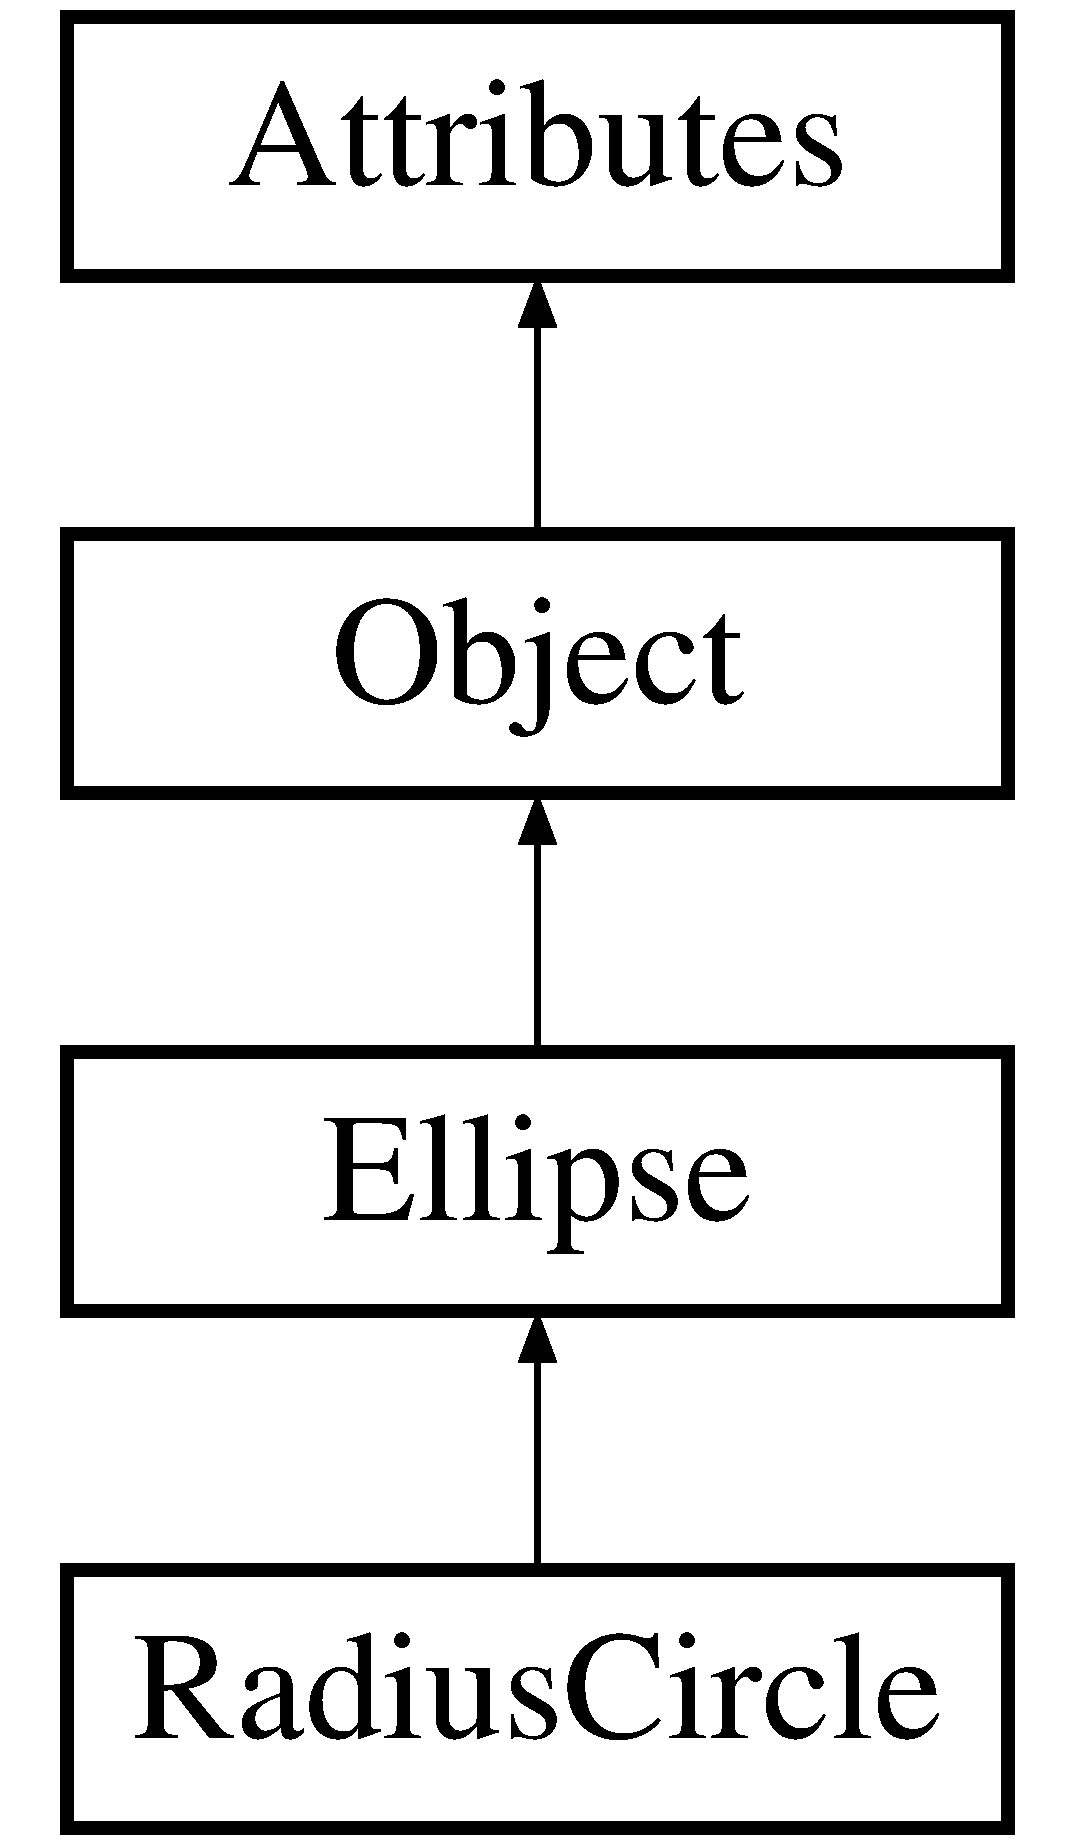
\includegraphics[height=4cm]{classRadiusCircle}
\end{center}
\end{figure}
\subsection*{Public Methods}
\begin{CompactItemize}
\item 
{\bf Radius\-Circle} ()
\item 
{\bf Radius\-Circle} ({\bf Coordinate} $\ast$, int)
\item 
{\bf $\sim$Radius\-Circle} ()
\end{CompactItemize}


\subsection{Detailed Description}
This class handles circles defined by their center and radius. This class is derived from {\bf Ellipse} {\rm (p.\,\pageref{classEllipse})}. \begin{Desc}
\item[Author: ]\par
Anthony Liekens \end{Desc}




\subsection{Constructor \& Destructor Documentation}
\index{RadiusCircle@{Radius\-Circle}!RadiusCircle@{RadiusCircle}}
\index{RadiusCircle@{RadiusCircle}!RadiusCircle@{Radius\-Circle}}
\subsubsection{\setlength{\rightskip}{0pt plus 5cm}Radius\-Circle::Radius\-Circle ()}\label{classRadiusCircle_a0}


\index{RadiusCircle@{Radius\-Circle}!RadiusCircle@{RadiusCircle}}
\index{RadiusCircle@{RadiusCircle}!RadiusCircle@{Radius\-Circle}}
\subsubsection{\setlength{\rightskip}{0pt plus 5cm}Radius\-Circle::Radius\-Circle ({\bf Coordinate} $\ast$, int)}\label{classRadiusCircle_a1}


\index{RadiusCircle@{Radius\-Circle}!~RadiusCircle@{$\sim$RadiusCircle}}
\index{~RadiusCircle@{$\sim$RadiusCircle}!RadiusCircle@{Radius\-Circle}}
\subsubsection{\setlength{\rightskip}{0pt plus 5cm}Radius\-Circle::$\sim$Radius\-Circle ()}\label{classRadiusCircle_a2}




The documentation for this class was generated from the following files:\begin{CompactItemize}
\item 
{\bf radiuscircle.h}\item 
{\bf radiuscircle.cpp}\end{CompactItemize}
